\subsection*{Punto 02}

\textbf{Genere un conjunto de datos de validación del mismo tamaño que el conjunto de entrenamiento y de la misma manera. Para cada k, asigne cada punto o dato de validación a la media de clúster aprendida más cercana en la parte (a) y muestre en una gráfica el valor de la función objetivo resultante de k-medias usando los datos de validación como una función de k. Comenta lo que ves. Qué valor de k se seleccionaría si usara como criterio de selección el minimo valor de la funcion objetivo para los datos de validación?}

En la figura \ref{fig:problema_03_validation_scores} se muestra los resultados de la función objetivo para los datos de validación. Si se usará el criterio del valor mínimo de la función de objetivo el k seleccionado sería el k=14. En la tabla \ref{table:problema_3_minimum_cost} se muestran los cinco k con menor valor en la función objetivo.

\begin{figure}[H]
    \centering
    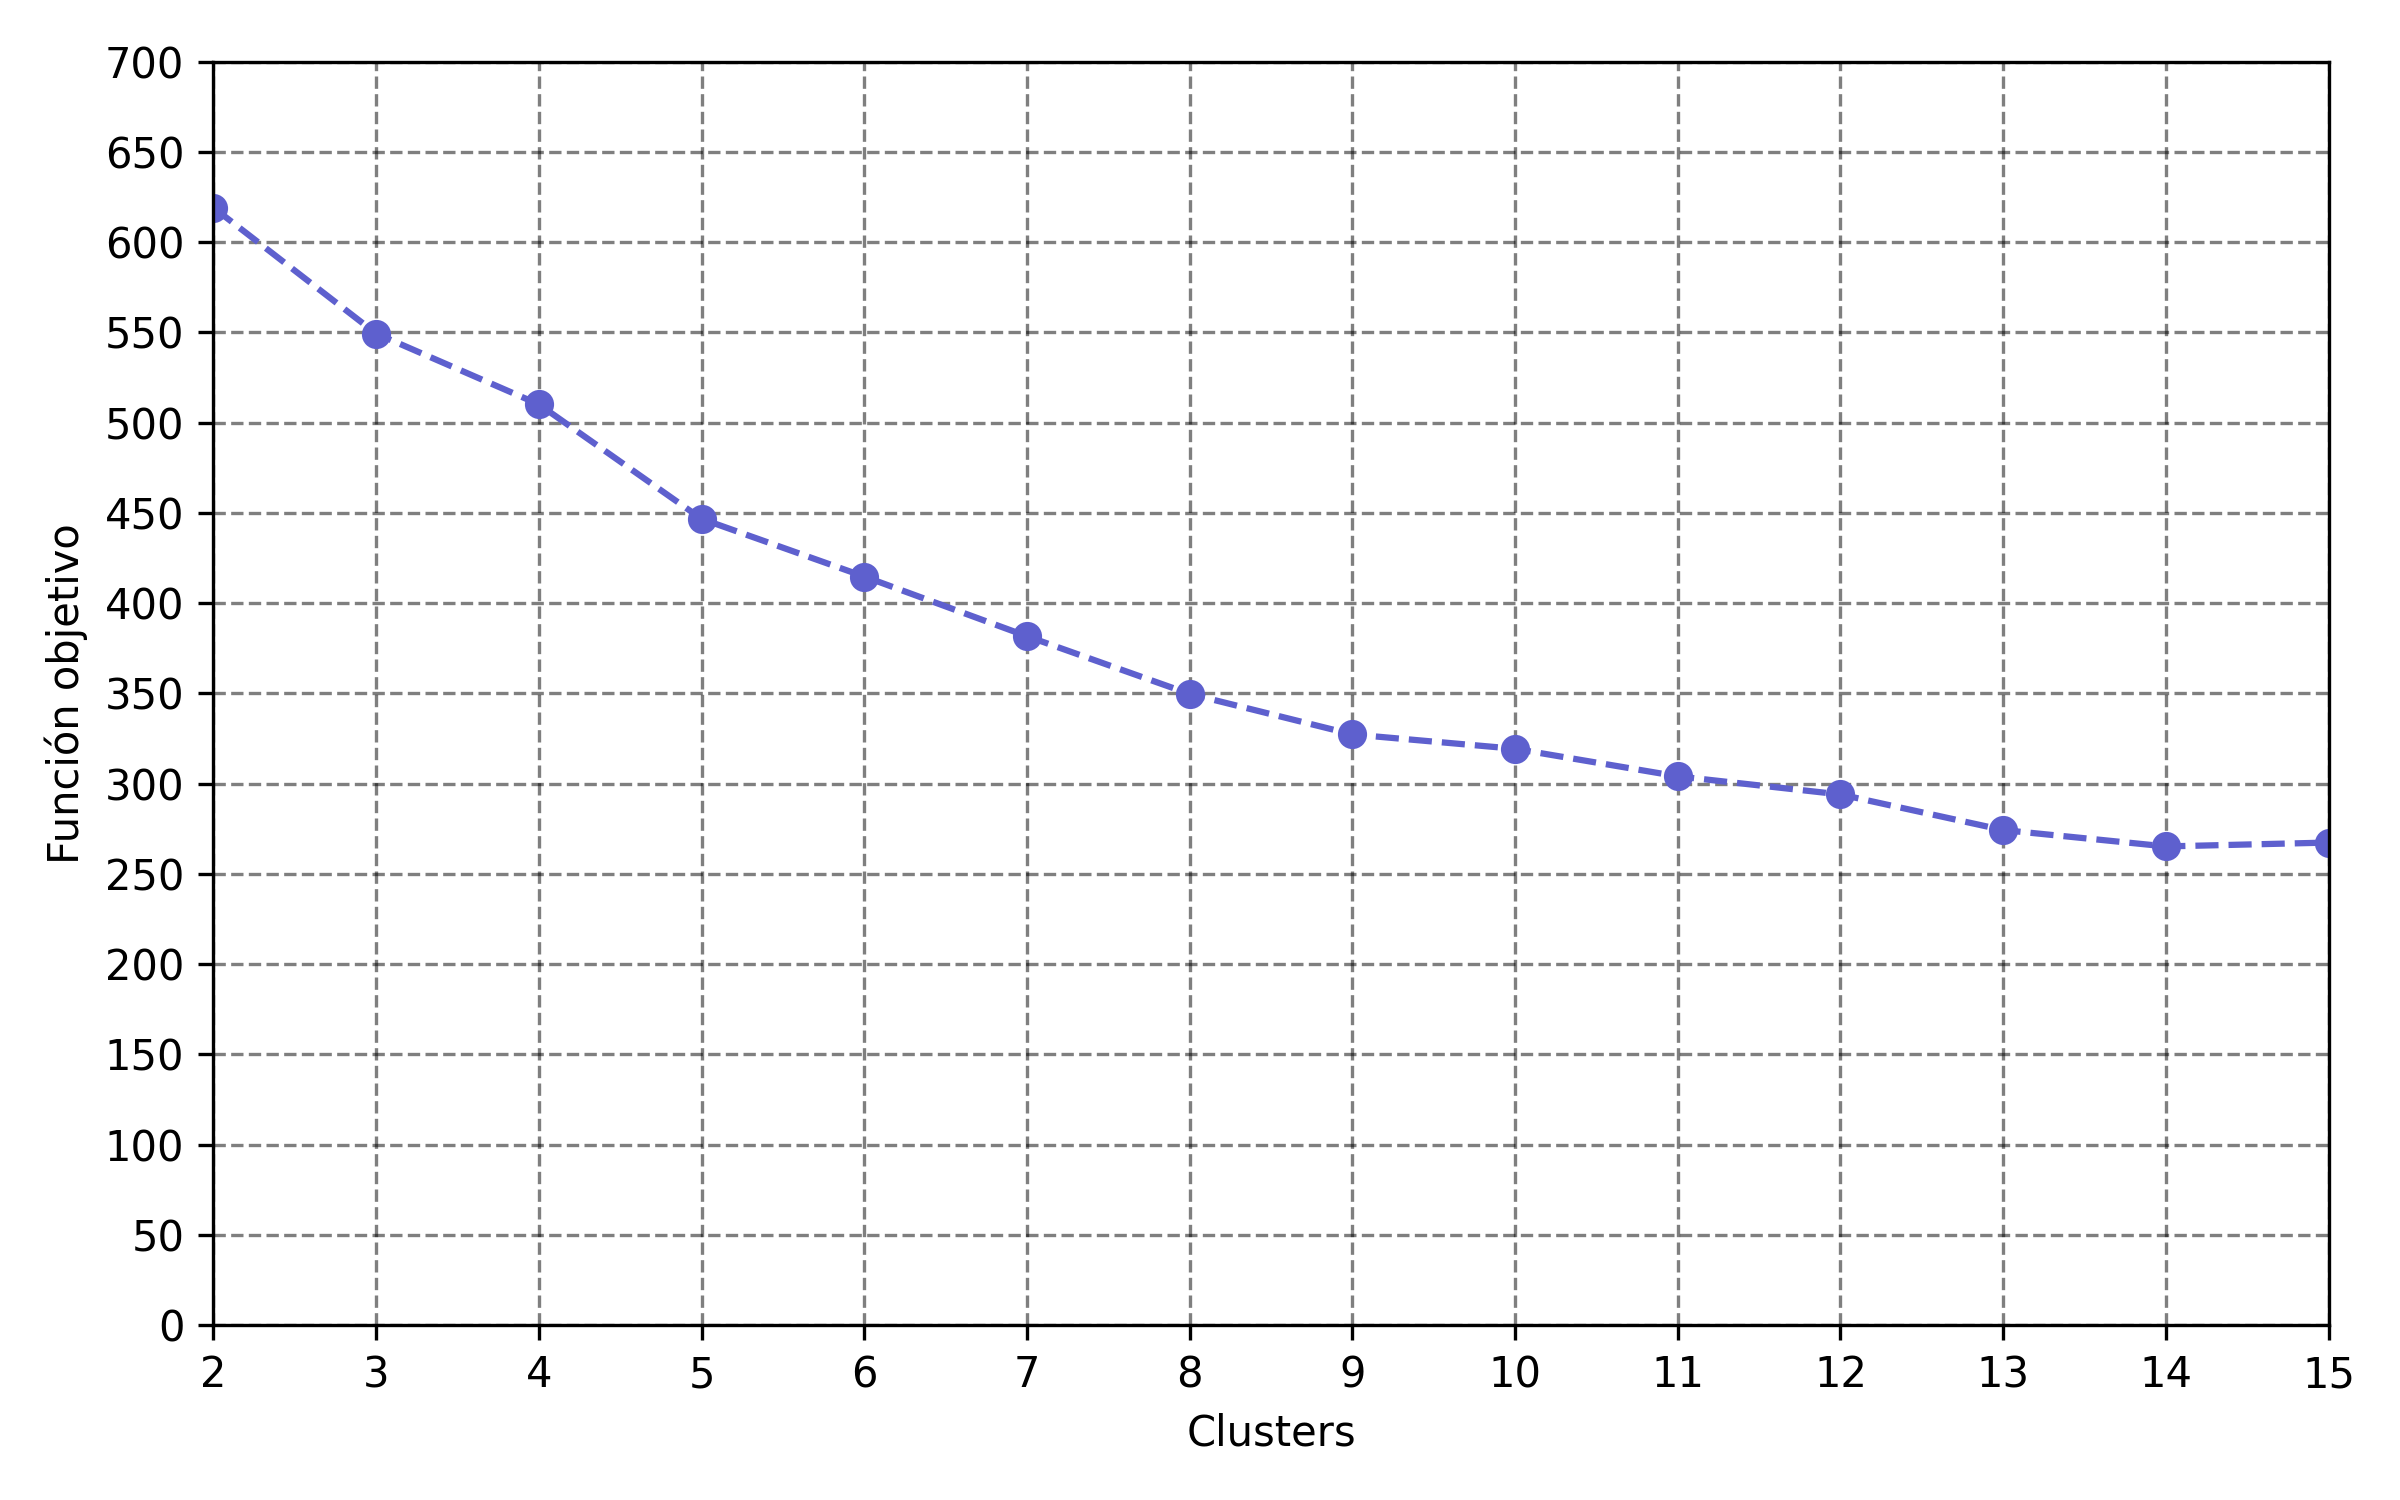
\includegraphics[width=14cm]{Graphics/Problema_03/validation_scores.png}
    \caption{Valor de la función objetivo para los datos de validación.}
    \label{fig:problema_03_validation_scores}
\end{figure}

\begin{table}[H]
    \centering
    \begin{tabular}{cc} \hline
        $k$ & \textbf{Función objetivo} \\ \hline
        14  & 265.194122                \\
        15  & 267.335407                \\
        13  & 274.270514                \\
        12  & 293.978512                \\
        11  & 304.018999                \\ \hline
    \end{tabular}
    \caption{Valores de k con menor costo objetivo.}
    \label{table:problema_3_minimum_cost}
\end{table}